\documentclass[a4paper,14pt]{article}
\usepackage{filecontents}

\usepackage[utf8]{inputenc}
\usepackage[english]{babel}
\usepackage{graphicx, array, blindtext}
\usepackage[colorinlistoftodos]{todonotes}
\DeclareUnicodeCharacter{2212}{-}
\usepackage [a4 paper , hmargin = 1.2 in , bottom = 1.5 in] {geometry}
\usepackage [parfill] {parskip}

\usepackage{enumitem}
\usepackage{amsmath}
\usepackage{amsthm}

\usepackage{nameref}
\usepackage{amssymb}
\usepackage [linesnumbered, ruled, vlined] {algorithm2e}
\usepackage{listings}
\usepackage{xcolor}
\usepackage{floatrow}
\usepackage{siunitx}
\usepackage{cancel}
\usepackage{fancyhdr}
\usepackage{graphicx}
\usepackage{verbatim}
\usepackage{color, colortbl}
\definecolor{highlight}{rgb}{0.75,1,1}
\usepackage[document]{ragged2e}

\renewcommand{\footrulewidth}{0.4pt}
\newtheorem{definition}{Definition}
\numberwithin{definition}{section}
\newtheorem{mytheorem}{Theorem}
\numberwithin{mytheorem}{subsection}
\newcommand{\notimplies}{\;\not\!\!\!\longrightarrow}  
\newcommand\norm[1]{\left\lVert#1\right\rVert}
\pagestyle{fancy}
\fancyhf{}
\rhead{CS754 Assignment 4}
\lhead{200050013-200050130}
\fancyfoot[C]{Page \thepage}
\usepackage{subcaption}
\usepackage{listings}


\usepackage{hyperref}
\urlstyle{same}
\hypersetup{pdftitle={main.pdf},
    colorlinks=false,
    linkbordercolor=red
}
\usepackage{array}
\usepackage{listings,chngcntr}

\begin{document}
\centering{

\title{\fontsize{150}{60}{CS754 Assignment 4 Report}}

\author{
Arpon Basu \\ Shashwat Garg }
}

\date{Spring 2022}
\maketitle

\justifying
\tableofcontents

\newpage
\justifying
\section*{Introduction}

Welcome  to our report on CS754 Assignment 4. We have tried to make this report comprehensive and self-contained. We hope reading this would give you a proper flowing description of our work, methods used and the results obtained.

Also note that we installed the \texttt{Image Processing Toolbox} in MATLAB for this assignment. Thus the grader is urged to install it if she wishes to run the code on her on her machine. Also note that some of our code may take a while to run because of the intensive nature of the computations involved.

Hope you enjoy reading the report. Here we go!
\section{Problem 1}


In this problem, we try out the cross validation technique and see if we can train and find an optimal value of lambda and then test that value for images that are not in our trained set. This is a very popular technique in machine learning and gives us a measure of robustness of our estimate


\subsection{Plots and Graphs of RMSE and VE}

\begin{center}
    \begin{tabular}{|c|c|c|}
        \hline
        Lambda	&	RMSE  &	Validation Error\\
        \hline
        0.0001  &  0.0061 &   2.5425\\
        0.0005  & 0.0061  &  2.5421\\
        0.0010  &  0.0061 &   2.5414\\
        0.0050  &  0.0061 &  2.5573\\
        0.0100  &  0.0061 &  2.5517\\
        0.0500  &  0.0060 &   2.5378\\
        0.1000  & 0.0059  &  2.5237\\
        0.5000  &  0.0050 &   2.0632\\
        1.0000  &  0.0044 &   1.7882\\
        \hline
        \rowcolor{highlight}
        2.0000  &  0.0040 &   1.6477\\
        \hline
        5.0000  &  0.0054 &   2.0351\\
       10.0000  &  0.0101 &   3.9400\\
       15.0000  &  0.0143 &   6.5897\\
       20.0000  &  0.0190 &  10.4407\\
       30.0000  &  0.0283 &  21.2658\\
       50.0000  &  0.0470 &  54.3791\\
      100.0000  &  0.0901 & 187.8113\\
        \hline
    \end{tabular}
    \end{center}


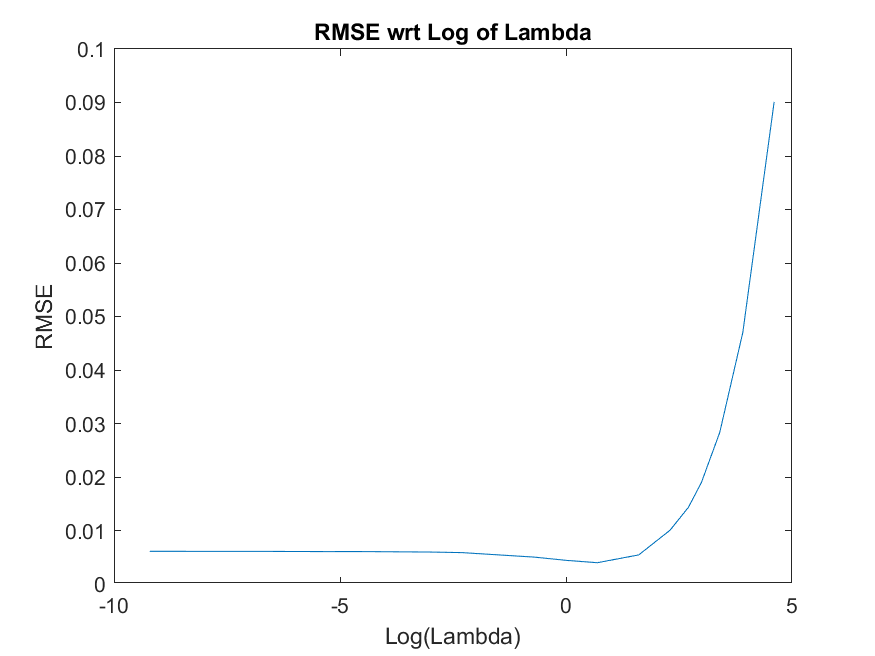
\includegraphics[width=7cm]{RMSE.png}
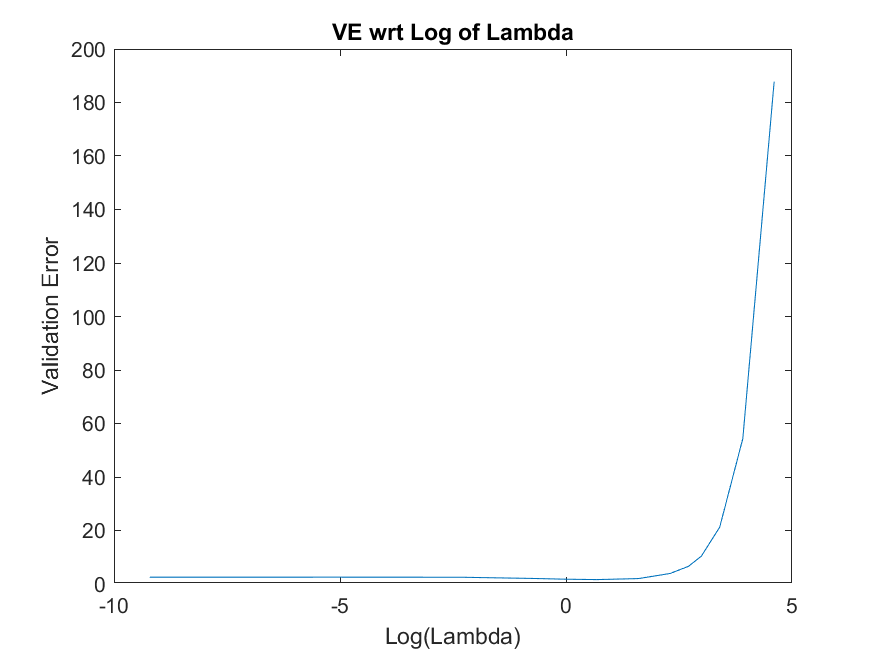
\includegraphics[width=7cm]{VE.png}

As you can see in the above graphs, the trend of both RMSE and Validation Error matches strongly. At $\lambda=2$, both the RMSE and VE are at their minimum value. Thus, we can say that our estimates of lambda on the trained set are robust. This is because they match the optimal behaviour also on the new unseen images.

\subsection{Coincident V and R}

The whole method of cross validation is made to simulate/test out our method in real life like scenarios, where the compressive system would encounter new images, but of the same type/distribution. Since we already train over the R set, there is no point of the V set if it is the same as R.

The Validation error would just be a scaled version of the RMSE. We would not know if we have \textbf{underfitted} or \textbf{overfitted} to our training set.

In case we are performing cross-validation, it is extremely important to keep the R and V sets of the same distribution for any accurate results, but also disjoint, so as to actually test out the performance.

\subsection{Proxying Ability}




\subsection{Theoretical $\theta$ vs Cross Validation $\theta$}




\section{Problem 2}
Let $D = \{d_1, d_2, ..., d_n\}$ be our dictionary, and let $I\in\mathcal{S}$ be an image in our dataset. Then by the theory of dictionary learning, $I = \sum^{n}_{i = 1}\alpha_id_i$ for some sequence of scalars $\alpha_1$, $\alpha_2$, $\hdots$, $\alpha_n$. In this problem, we are given various transformations $T$ which are applied on the images of $\mathcal{S}$, and we have to propose a modified dictionary $D_T$ such that our transformed images are still expressible as linear combination of ``atoms" in $D_T$.\\
(a) From the theory taught in class and common image processing literature, we know that derivative filters on an image are obtained through \textbf{convolutions} of the image with some known convolution filter, ie:- $I_{\mathrm{filter}} = I * G$, where $G$ is the filter matrix. Now, it's not hard to see that a matrix convolution is a linear mapping, ie:- the \textbf{derivative filter `$f$' is itself a linear transform} on the image.Then 
$$f(I) = f(\sum^{n}_{i = 1}\alpha_id_i) = \sum^{n}_{i = 1}f(\alpha_id_i) = \sum^{n}_{i = 1}\alpha_if(d_i)$$
where all the equalities follow by the properties of linear transforms.\\
\textbf{Thus our transformed dictionary is $D_T := \{f(d_1), f(d_2), \hdots, f(d_n)\}$, where $f$ represents our derivative filter.}
\\
(b) Once again, note that rotation is a linear transform. In particular, the rotation of an image (matrix) $I$ anticlockwise by an angle $\theta$ can be given as below
$$I_{\mathrm{rotated}}(x, y) = I(x\cos\theta+y\sin\theta, y\cos\theta-x\sin\theta)$$
or equivalently as
$$I_{\mathrm{rotated}}([x\;\;y]^T) = I(R_{\theta}^{-1}[x\;\;y]^T)$$
where the rotation matrix $R_{\theta}$ represents anticlockwise rotation by an angle $\theta$
$$R_{\theta} = \begin{bmatrix}
    \cos\theta \;\; -\sin\theta\\
\sin\theta \;\; \cos\theta
\end{bmatrix}$$ 
\\
Thus, once again, we have a linear transform in our hands and thus the new atoms of our transformed dictionary will just be the linear transform applied on the old dictionary itself, ie:- rotated versions of the old atoms. We will have two such dictionaries (for two distinct angles of rotation). Note that we must take the union of both dictionaries as an image, say rotated by $\beta$ won't be expressible as a linear combination of dictionary atoms rotated by the angle $\alpha$.\\
\textbf{Thus our transformed dictionary is $D_T := \{d_{1\alpha}, d_{2\alpha}, \hdots, d_{n\alpha}, d_{1\beta}, d_{2\beta}, \hdots, d_{n\beta}\}$, where $d_{k\theta}$ represents the $k^{\mathrm{th}}$ atom rotated by $\theta$.}
\\
(c) Assuming the relation holds pixel-wise, we have
$$I_{\mathrm{new}}(x,y) = \alpha(I_{\mathrm{old}}(x,y))^2 + \beta I_{\mathrm{old}}(x,y) + \gamma$$
But we have
$$I_{\mathrm{old}}(x,y) = \sum^{n}_{i = 1}\alpha_id_i(x,y)$$
$$\implies I_{\mathrm{new}}(x,y) = \alpha(\sum_{i=1}^{n} \alpha_id_{i}(x,y))^2+\beta\sum_{i=1}^{n} \alpha_id_{i}(x,y)+\gamma $$
$$\implies I_{\mathrm{new}}(x,y) = \alpha(\sum_{i=1}^{n} \alpha_i^2d_{i}^2(x,y) + 2\sum_{1\leq i < j\leq n}\alpha_i\alpha_jd_{i}(x,y)d_{j}(x,y))+\beta\sum_{i=1}^{n} \alpha_id_{i}(x,y)+\gamma $$
Thus our new dictionary is clear:
\begin{itemize}
    \item First class of items: $\{d_1^{\circ 2}, d_2^{\circ 2}, ..., d_n^{\circ 2}\}$, where $^{\circ 2}$ denotes \textbf{elementwise squaring}.
    \item Second class of items: $\{d_i\odot d_j\}_{1\leq i < j\leq n}$, where $\odot$ denotes \textbf{elementwise multiplication}.
    \item Third item: $J_{d\times d}$, where $d_i\in\mathbb{R}^{d\times d}$, where $J$ is the matrix of all ones, ie:- $J = \;$\texttt{ones(d)}, in MATLAB notation.
\end{itemize}
\textbf{Thus our transformed dictionary is $D_T := \{d_1^{\circ 2}, d_2^{\circ 2}, ..., d_n^{\circ 2}, d_1\odot d_2,\hdots,d_{n-1}\odot d_{n},J_{d\times d}\}$.}
\\
(d) Blur kernel, like derivative filters, are also convolutions with kernel matrices and hence are linear transforms.\\
\textbf{Thus our transformed dictionary is $D_T := \{f(d_1), f(d_2), \hdots, f(d_n)\}$, where $f$ represents our blur kernel transformation.}
\\
(e) Similar to the idea used in part (b), we have to take an union of all the dictionaries, each applied with a single blur kernel. Thus let $\mathcal{B} := \{b_1, b_2, ..., b_l\}$ be the set of our blur \emph{transforms}. Then our $l$ dictionaries are $\{b_1(d_1), b_1(d_2), \hdots, b_1(d_n)\}$, $\{b_2(d_1), b_2(d_2), \hdots, b_2(d_n)\}$, ..., $\{b_l(d_1), b_l(d_2), \hdots, b_l(d_n)\}$, and \\
\textbf{Thus our final dictionary is $D_T$
 $:= \{b_1(d_1), \hdots, b_1(d_n), \hdots, b_l(d_1), b_l(d_2), \hdots, b_l(d_n)\}$.}\\
(f) Note that the meaning of the notation for this part is slightly different from all other parts of this problem in the fact that our images and dictionary atoms are now assumed to the vectorized forms of the images they represented. Now, note that the Radon transform matrix can be denoted as $R_{\theta}$, which is a square matrix with entries dependent on $\theta$, which when multiplied with our image vectors gives us their Radon transform. Once again, as above, since this is a linear transform of the vectors, our new dictionary will be the Radon transform of the dictionary atoms. \textbf{Thus our new dictionary $D_T := \{Rd_1, Rd_2, \hdots, Rd_n\}$, where $R$ is the Radon transform matrix corresponding to the angle $\theta$.}\\
(g) Note that translating an image by a certain offset $(x, y)$ basically means that we \textbf{pad the image, on the left and downwards, with $x$ columns and $y$ rows of zeros respectively}. Now, since we simply added an extra layer of padding of zeros, the linear combination relations still hold as the zero rows and columns obviously satisfy any linear relation and the old pixels also satisfy the relation too. Thus if we denote translation by the first offset to be $t_1$ and the second offset to be $t_2$, then, as we have seen many times before our \textbf{new dictionary will be $D_T$
$:= \{t_1(d_1), \hdots, t_1(d_n), t_2(d_1), t_2(d_2), \hdots, t_2(d_n)\}$.}
\section{Problem 3}
\subsection{Part 1}
We use the \textbf{Eckart-Young-Mirsky theorem} to find the \textbf{best rank $r$ approximation to the given matrix $A\in\mathbb{R}^{m\times n}$}, ie:- $A_r$, which, as we have seen in the lecture, states that the best (in terms of the Frobenius norm of the difference in between those two matrices) $r$-rank approximation is given by $A_r = U\Sigma_rV^*$, where $A = U\Sigma V^*$ is the \textbf{Singular Value Decomposition} of $A$, and $\Sigma_r$ contains the $r$ maximum singular values in $\Sigma$, ie:- we retain the $r$ largest diagonal values of $\Sigma$ and set the rest to zero.\\
Thus the minimizer of the objective function $J(A_r) = \lVert A - A_r\rVert^2_F$; rank$(A_r) = r$ is 
$$\boldsymbol{A_r = U\Sigma_rV^*}$$
where $A = U\Sigma V^*$ is the SVD decomposition of $A$ and $\Sigma_r$ contains the $r$ maximum singular values in $\Sigma$.\\
Applications of low rank approximations:
\begin{itemize}
    % \item \textbf{Recommender Systems:} Many a times matrices \textbf{with very few known entries} need to be completed based on the knowledge that the matrix has a low rank. Such approximations are useful there.
    % \item \textbf{Denoising:} In many systems, noise may artificially increase the rank of the original matrix which was otherwise low rank. Low rank approximations of the noisy matrix will thus resemble the actual matrix as they will filter much of the noise out.
    \item \textbf{Robust PCA}
    \begin{itemize}
        \item Note that in a surveillance video, the background remains stationary while our object of interest moves. Thus the background of the image can be treated as it's low rank component, which can then be identified using the algorithm outlined above.
        \item In a similar vein as the idea above, one can remove occlusion by \textbf{completing} a low rank matrix to effectively ``cut-out" the occluding object in the image.
    \end{itemize} 
\end{itemize}
\subsection{Part 2}
We algebraically simplify the objective function $J(R) = \lVert A - RB\rVert^2_F$ first to find out the optimum orthonormal $R$ matrix. For that, note the following facts from linear algebra:
\begin{itemize}
    \item $\lVert A\rVert^2_F = \;$tr$(AA^T)$
    \item tr$(AB)$ = tr$(BA)$, and thus any rearrangement of a matrix multiplication will still yield the same trace.
    \item tr($A$) = tr($A^T$) for any square matrix $A$
\end{itemize}
Then 
$$\lVert A - RB\rVert^2_F = \mathrm{tr}((A - RB)(A - RB)^T) = \mathrm{tr}((A - RB)(A^T - B^TR^T))$$
$$ = \mathrm{tr}(AA^T - RBA^T - AB^TR^T + RBB^TR^T)$$
$$ = \mathrm{tr}(AA^T) - \mathrm{tr}(RBA^T) - \mathrm{tr}((RBA^T)^T) + \mathrm{tr}(RBB^TR^T)$$
$$ = \mathrm{constant} - \mathrm{tr}(RBA^T) - \mathrm{tr}(RBA^T) + \mathrm{tr}(R^TRBB^T)$$
$$ = \mathrm{constant} - 2\cdot\mathrm{tr}(RBA^T) + \mathrm{tr}(BB^T)$$
$$ = \mathrm{constant} - 2\cdot\mathrm{tr}(RBA^T)$$
Thus minimizing $\lVert A - RB\rVert^2_F$ is equivalent to maximizing $\mathrm{tr}(RBA^T)$. \\
Now, let $BA^T$ be equal to $C$, and let $C = U\Sigma V^*$ be the \textbf{Singular Value Decomposition} of $C$.\\
Then
$$\mathrm{tr}(RBA^T) = \mathrm{tr}(RC) = \mathrm{tr}(RU\Sigma V^*) = \mathrm{tr}(V^*RU\Sigma)$$
Now, note that since $R$, $U$ and $V$ are all orthonormal, $M = V^*RU$ is orthonormal too, and thus 
$$\mathrm{tr}(V^*RU\Sigma) = \mathrm{tr}(M\Sigma) = \sum^{n}_{i = 1} m_{ii}\sigma_i\leq\sum^{n}_{i = 1} |m_{ii}|\sigma_i$$
with the last inequality following by the triangle inequality (and note that $|\sigma_i| = \sigma_i$ since singular values are non-negative).\\
However, since $M$ is orthonormal, ie:- all of it's column's norms are 1, we have that $|m_{ii}|\leq 1$, and thus the maxima of $\mathrm{tr}(V^*RU\Sigma)$ is achieved when all $|m_{ii}| = 1$. But that can happen only when $M = I$, and thus
$$V^*RU = I $$
$$\boldsymbol{\implies R = VU^*}$$
Thus the best orthonormal transform that maps $B$ to $A$ is given by $VU^*$, where $U$ and $V$ are obtained from the SVD of $BA^T = U\Sigma V^*$.\\
This problem is also widely encountered in image processing literature. We ourselves came across one such example in class, namely, in 3D Tomography under unknown angles, wherein we try to determine what rotation best maps one image to another, and there is where we note that orthonormal matrices basically represent unscaled rotation in higher dimensions, from which the problem of minimizing $\lVert A - RB\rVert^2_F$ under an orthonormal $R$ constraint arises.


\section{Problem 4}












































\section{Problem 5}
Note that we have to find the $f$ vector which is most likely to have arisen from the $y$ vector we know under the equation $y$ $\sim$ Poisson$(I_0e^{-Rf})$, where all the operations are done element-wise on the vectors. Note that $R$ is the \textbf{known} Radon matrix.\\
Stating this mathematically, we want
$$f = \mathrm{arg}\;\mathrm{max}_{f \in \mathbb{R}^m} P(f|y)$$
Now, note that $P(f|y) \propto P(y|f)P(f)$ by Baye's theorem, where $P(f)$ is a \textbf{prior} on $f$, ie:- a probability distribution on $\mathbb{R}^m$ which tells us how likely a certain point in $\mathbb{R}^m$ is to represent the natural tissue density vector.\\
But before specifying the functional form of the prior, we'll simplify $P(y|f)$ a bit. Also note that maximizing a certain non-negative function (such as a probability distribution) is equivalent to minimizing it's negative logarithm.\\
Note that since $y$ varies with $f$ as a Poisson relation
$$P(y|f) = \frac{e^{I_0e^{-Rf}}(I_0e^{-Rf})^y}{y!}$$
$$\implies -\log P(y|f) = I_0e^{-Rf} - y\log (I_0e^{-Rf}) + \log (y!)$$
$$\implies -\log P(y|f) = \lVert I_0e^{-Rf}\rVert_1 + y^TRf$$
where we drop all terms not having $f$ in them because we're to define an objective function dependent on $f$. Note also that we transpose $y$ at the end to make the matrices multipliable. Also note that to convert the vector $I_0e^{-Rf}$ to a scalar, we take its $l_1$ norm (note also that the $l_1$ norm promotes sparsity, which is a desirable quality to have for our objective function), because $y^TRf$ is also a scalar, and we need to add them both.\\
Now coming to the prior, note that $f$ denotes natural tissue density. Now, from our study of natural images and other naturally arising phenomena, we know that \textbf{their gradients are sparse}. This is only to be expected since consecutive entries for the most part don't change rapidly.\\
Thus, if we define the \textbf{gradient of a vector as follows}
$$\nabla f := \sum^{m - 1}_{i = 1} |f_i - f_{i + 1}|$$
Then
$$P(f) \propto e^{-\nabla f} $$
is a suitable prior. Taking it's negative logarithm we get 
$$-\log P(f) = \nabla f$$, and thus
$$-\log P(f|y) = -\log P(y|f) -\log P(f)$$
$$-\log P(f|y) = \lVert I_0e^{-Rf}\rVert_1 + y^TRf + \mu\nabla f$$
where $\mu$ is a suitable hyperparameter denoting the importance of how much the gradient sparsity is to be tuned.\\
% But note that this quantity is still a vector, and we want to make it as small as possible, in the sense that each of it's entries should as close to zero as possible. 
Thus
$$\boldsymbol{J(f) := \lVert I_0e^{-Rf}\rVert_1 + y^TRf + \mu\nabla f}$$
Finally, note that for additive white Gaussian noise, we can simply minimize the mean square error (unlike Poisson noise, Gaussian noise is independent of the pixel value it distorts, and thus minimizing the mean square error should suffice). Note that the mean of a Poisson RV is equal to it's parameter, and thus $y$ should be compared to $I_0e^{-Rf}$, and thus 
$$\boldsymbol{J_{\mathrm{Gaussian}}(f) := \lVert y - I_0e^{-Rf}\rVert^2_2}$$
Combining these two together
$$\boldsymbol{J_{\mathrm{complete}}(f) := \lVert I_0e^{-Rf}\rVert_1 + y^TRf + \mu\nabla f + \lambda\lVert y - I_0e^{-Rf}\rVert^2_2}$$
where $\lambda$ is another hyperparameter to stress the importance of the Gaussian error function.
\end{document}